\documentclass{article}

% if you need to pass options to natbib, use, e.g.:
%     \PassOptionsToPackage{numbers, compress}{natbib}
% before loading neurips_2021

% ready for submission
\usepackage{neurips_2021}



% to compile a preprint version, e.g., for submission to arXiv, add add the
% [preprint] option:
%     \usepackage[preprint]{neurips_2021}

% to compile a camera-ready version, add the [final] option, e.g.:
%     \usepackage[final]{neurips_2021}

% to avoid loading the natbib package, add option nonatbib:
%    \usepackage[nonatbib]{neurips_2021}

\usepackage[utf8]{inputenc} % allow utf-8 input
\usepackage[T1]{fontenc}    % use 8-bit T1 fonts
\usepackage{hyperref}       % hyperlinks
\usepackage{url}            % simple URL typesetting
\usepackage{booktabs}       % professional-quality tables
\usepackage{amsfonts}       % blackboard math symbols
\usepackage{nicefrac}       % compact symbols for 1/2, etc.
\usepackage{microtype}      % microtypography
\usepackage{xcolor}         % colors

% custom imports
\usepackage{mystyle}
\usepackage{algorithm}
\usepackage[noend]{algorithmic}
\newcommand\todo[1]{\textcolor{red}{#1}}
\usepackage{subcaption}
\usepackage{multirow}

\title{Embedded Structured Prediction}

% The \author macro works with any number of authors. There are two commands
% used to separate the names and addresses of multiple authors: \And and \AND.
%
% Using \And between authors leaves it to LaTeX to determine where to break the
% lines. Using \AND forces a line break at that point. So, if LaTeX puts 3 of 4
% authors names on the first line, and the last on the second line, try using
% \AND instead of \And before the third author name.

\author{%
  David S.~Hippocampus\thanks{Use footnote for providing further information
    about author (webpage, alternative address)---\emph{not} for acknowledging
    funding agencies.} \\
  Department of Computer Science\\
  Cranberry-Lemon University\\
  Pittsburgh, PA 15213 \\
  \texttt{hippo@cs.cranberry-lemon.edu} \\
  % examples of more authors
  % \And
  % Yuntian Deng \\
  % Affiliation \\
  % Address \\
  % \texttt{email} \\
  % \AND
  % Alexander M. Rush \\
  % Affiliation \\
  % Address \\
  % \texttt{email} \\
}

\begin{document}

\maketitle

\begin{abstract}
  Structured distributions, i.e. distributions over combinatorial
  spaces, allow for more flexible latent probabilistic representations
  compared to simple fixed-size categorical distributions. However,
  scaling these models is bottlenecked by the high computational and
  memory complexity with respect to the number of hidden states.  Classical models
  such as Hidden Markov Models (HMMs) and Probabilistic Context-Free
  Grammars (PCFGs) require time and space quadratic and cubic in the
  number of hidden states respectively.  This work demonstrates a
  simple approach to reduce the computational and memory complexity of
  a large class of structured models. We show that by kernelizing the
  central belief propagation step in inference we can reduce
  complexity by a factor of the hidden state size, critical when scaling to
  large models. To take advantage of this approach with effective
  structured parameterizations, we apply recent approaches to softmax
  kernel approximation. This method provides exact inference for a
  model approximation of standard structured distributions.
  Experiments on language modeling and unsupervised grammar induction
  show that our approach matches the accuracy of standard models, 
  while also scaling to very large state spaces.
\end{abstract}


\section{Introduction}

% what is structured prediction

Learning flexible latent representations from data has become a
critical component of modern semi-supervised learning. Typically
models for tasks like natural language processing (NLP) are trained on
large sets of unsupervised data to learn potential internal structures
that can be transferred to new tasks \citep{devlin2018bert,radford2019language,liu2019roberta}.
The dominant paradigm in this
space is to learn a large, opaque neural network, such as a
transformer, and have it parameterize a simple output distribution,
typically a fixed-sized softmax categorical.

Why have the neural representations in these models continued to evolve,
while the probabilistic output component of the model has remained relatively
simple? We posit that a major issue is computational complexity.  Any
discrete model richer than a softmax begins to incur large asymptotic
costs in training and inference. Any benefits from latent probabilistic
structure are overwhelmed by practical scale.

Two canonical \textit{structured} models used in NLP are Hidden Markov
Models (HMMs) and Probabilistic Context-Free Grammar (PCFGs). These models
incorporate relatively simple probabilistic dependencies: HMMs along
the surface and PCFGs in a hierarchical manner.  With enough latent
capacity and training data, one might expect these models to learn non-trivial
representations, while preserving the ability to compute posterior
distributions. However, the runtime of training HMMs and CFGs scales 
quadratically and cubically in the number of states respectively,
which limits their use to prohibitively small models.


% In particular discrete
% latent-variable models scale poorly in the number of states.



% Indeed, a key component of structured prediction algorithms is balancing model expressivity with the computational cost of inference, since complex models are necessary to fit the large-scale datasets that are common in machine learning.
% Furthermore, incorporating latent variables, which increase models expressivity and are necessary for modeling unobserved phenomena, result in an even larger inferential burden.
% Much work in machine learning seeks to find a desirable point in the tradeoff between model complexity and cost of inference.

% While structured models offer interpretability, this comes at
% a cost: an increase in model complexity comes with an associated
% increase in the cost of inference.

% Structured prediction , such as language modeling, often require models to capture and learn complex dependencies, both observed and unobserved.
% One approach to structured prediction is to offload the burden of learning these dependencies to an expressive black-box \todo{neural?} model, often obtaining high accuracy at the cost of forgoing the ability to examine the learned dependencies.
% Another approach is to learn a structured model, where the dependencies are specified explicitly.
% \todo{More on what structured models are?}
% While structured models offer interpretability, this comes at a cost: an increase in model complexity comes with an associated increase in the cost of inference.

% structured prediction: accuracy vs complexity tradeoff

% Recent work in computationally efficient atte
This work targets these issues with a method for
\textit{embedded structured prediction} that improves on the asymptotic complexity
of structured models like HMMs and CFGs
without sacrificing empirical accuracy.
We consider models in the
formalism of labeled directed hypergraphs which describes a broad class
of structured inference \citep{klein2004parsing,huang2005better,zhou2006learning,javidian2020hypergraph,chiang2020factor}.
We show how applying a low-rank kernel
decomposition constraint greatly increases the speed of inference.
This approach builds on work in approximate belief propagation in non-parametric
graphical models~\citep{song2011kernelbp}.

Starting with this decomposition, we develop new models that approximate
standard neural structured models. Our approach applies recent work in
computationally efficient neural attention models~\citep{peng2021rfa,choromanski2020performer}.
The key ingredient in these, seemingly unrelated, approaches is a specific
low-rank kernel parameterization that rewrites neural attention from a large
softmax to a low-dimensional embedded feature map representation.
With a low-rank kernelized
inference representation, we can directly extend these advances to the
structured prediction setting.

We evaluate this approach to embedded structured prediction by
applying kernelization to a language modeling task with HMMs and PCFGs.
The application of kernelization is
nontrivial in high-dimensional structured models, and we demonstrate
effective techniques for overcoming several practical challenges.
We find that our approach achieves
very similar results compared to exact structured models, while the
decomposition allows us to greatly increase the speed of inference.
Results on HMMs let us scale to more than 16,000 states, while PCFGs achieve 
a significant perplexity reduction compared to past work. 


\section{Background: Structured Prediction}

As motivation we consider the problem of modeling the joint distribution of
a sequence of tokens $p(x)= p(x_1, \dots, x_T)$.
We note that the most effective empirical approach is to model with an autoregressive neural network,
and to output the probability of each token as a categorical distribution.
While accurate, this approach hides much of its complexity in opaque neural parameters,
which can make it difficult to analyze or compose with other models.

We instead consider generative modeling based approaches that explicitly
utilize a hidden (latent) representation structure $z$, which may take various
forms depending on the application and model.
Structured models explicitly take into account correlations between variables by
modeling the joint distribution $p(x,z)$.

As we only observe $x$, we must optimize the evidence
$p(x) = \sum_z p(x,z)$ by marginalizing over $z$ to train a
structured model with latent variables. Scaling this marginalization
will be the focus of this work. Therefore before discussing the
specifics of the models we introduce general-purpose machinery for
performing this marginalization.

% Models of interest

\subsection{Inference with Hypergraphs}

Hypergraphs are a graphical model formalism that
unify a class of structured distributions that admit tractable
inference through dynamic programming \citep{klein2004parsing,huang2005better,zhou2006learning,javidian2020hypergraph,chiang2020factor}.
While the formalism is similar to undirected factor graphs,
it allows us to represent more complex distributions: notably
dependency structures with unknown topologies, such as trees.

We define a labeled, directed acyclic hypergraph as a set of nodes
$v \in \cal V$ each with a collection of labels ${\cal L}_v$; a set of
hyperedges $\cal E$; and a designated start node $S \in {\cal V}$. Each
hyperedge $e$ consists of a head node $u$ and tuple of tail nodes,
 $v_1 \ldots v_{|e|}$.
For simplicity, we will assume at most 2 tail nodes $v_1, v_2$ throughout.
Each hyperedge $e$
is associated with a score function $\psi_{e}(z_u, z_{1}, z_{2})$
where $z_u\in \mcL_u$, $z_{1} \in {\cal L}_{v_1}$,
and $z_{2} \in {\cal L}_{v_2}$.
Finally, we assume we have a topological ordering over the edges.

A hypergraph can be used to sum up the multiplicative scores along hyperpaths.
This is done through an inside-style dynamic programming or belief
propagation algorithm.
The main benefit of the graphical representation is that it clearly provides the
runtime complexity based on the structure of the hypergraph.
The general algorithm is as follows, with table $\alpha$ starting at 0, 
\begin{algorithm}
\begin{algorithmic} 
\FOR {$u \leftarrow v_1, v_2$ hyperedge $e$ in topological order}
\FOR {$z_u \in {\cal L}_u$ }
\STATE $\alpha_u(z_u) \stackrel{+}{\gets}  \displaystyle \sum_{z_1, z_2}  \psi_e(z_u, z_1, z_2) \  \alpha_{v_1}(z_1) \  \alpha_{v_1}(z_2)$
\ENDFOR
\ENDFOR
\STATE \textbf{return} $\sum_z \alpha_S(z)$
\end{algorithmic} 
\end{algorithm}

The resulting value represents the sum over structure scores. Counting
loops, the worst-case run-time complexity is
$O(|{\cal E}|\times |{\cal L}^*|^{|e^*|+1})$ where $|{\cal L}^*|$ is the 
largest label set and $|e^*|$ the max hyperedge tail size.

\subsection{Hypergraphs for Generative Models}

For discrete latent-variable models, hypergraphs provide a convenient
representation for performing marginal inference.  Analogous to converting
tree-structured Bayes' nets to factor graphs, we assume that each node
represents a latent variable and the labels represent its state space.
Assuming the model factors as a tree, local conditional probabilities
can be directly turned into potentials $\psi$. Observed variables, in
this case $x_1, \ldots, x_n$, can be directly incorporated into the
potentials.\footnote{Note though that unlike many graphical models,
hypergraphs do not assume that every node needs to be utilized.}


%Not though that unlike factor graphs these variables may not be used, i.e. the sample space of $Z_h$
%is ${\cal L}_h \cup \{\epsilon\}$.

Specifically this procedure yields an update rule of,

\[\alpha_u(z_u) \stackrel{+}{\gets} \displaystyle \sum_{z_1, z_2}  p(z_1, z_2 \mid z_u) \  \alpha_{v_1}(z_1) \  \alpha_{v_2}(z_2).\]

Under this setting, the hypergraph provides the probability of
marginalizing out the latent states $z$, i.e. $\sum_z p(x, z)$. This procedure is needed to train a structured model or to evaluate
it on unseen data. To make this approach concrete, we focus on two examples of structured
models in this work: hidden Markov models and probabilistic
context-free grammars.


\paragraph{Example: Hidden Markov Model}

HMMs are classical sequence models defined by the following generative process: first, a sequence of discrete latent states $z = (z_1, \ldots,z_T)$ with state space $\cal L$ are chosen as a Markov chain. Each state $z_t$ then emits a single observation $x_t$.
This yields the joint distribution,
\begin{equation}
\label{eqn:hmm}
    p(x,z) = \prod_{t=1}^T p(z_t \mid z_{t-1})\ p(x_t\mid z_t),
\end{equation}
where $p(z_t \mid z_{t-1})$ is the transition distribution,
 $p(x_t \mid z_t)$ the emission distribution, and $p(z_1 \mid z_0)$ is 
the initial distribution.

Given a sequence of observations $x_1 \ldots x_n$ we can compute 
$p(x_1, \ldots, x_n)$ using a labeled directed hypergraph, with nodes corresponding to state positions, and emissions incorporated into the edge scores $\psi$. 

\begin{algorithm}
\begin{algorithmic} 
\FOR {$t \leftarrow (t+1)$ in right-to-left order}
\FOR {$z_t \in {\cal L}$ }
\STATE $\alpha_t(z_t) \stackrel{+}{\gets}  \displaystyle \sum_{z_{t+1}}  p(z_{t+1}, x_t \mid z_{t}) \  \alpha_{t}(z_{t+1})$
\ENDFOR
\ENDFOR
\STATE \textbf{return} $\sum_{z_0} \alpha_0(z_0)$
\end{algorithmic} 
\end{algorithm}


%\[\alpha_{t}(z_{t}) \gets \displaystyle \sum_{z_{t+1}}  p(z_{t+1}, x_t \mid z_{t}) \  \alpha_{t}(z_{t-1})\]


Inference on this graph corresponds to summing out over the latent structures $z$, i.e. 
computing $\sum_{z_{1:T}} p(z_{1:T}, x_1, \ldots, x_T) = p(x_1, \ldots, x_T)$. We 
can read off the derivation that this requires: time $O(T \times {|\cal L|}^2)$. This approach is identical to the backward algorithm for HMMs.

\paragraph{Example: Context-Free Grammars}


Context-free grammars (CFGs) are a structured model defined by the 5-tuple 
$\mcG = (S,\mcN,\mcP,\mcX,\mcR)$, where $S$ is the distinguished start symbol, $\mcN$ is a finite set of nonterminals, $\mcP$ is a finite set of preterminals, $\mcX$ is the elements in the output space, and $\mcR$ is a finite set of transition rules.
Rules take the form,
\begin{equation}
\label{eqn:pcfg-rules}
\begin{aligned}
S&\to A, & A\in\mcN,\\
A&\to B\ C, & B,C\in\mcN\cup\mcP,\\
T&\to x, & T \in\mcP,x\in\mcX.
\end{aligned}
\end{equation}
A probabilistic context-free grammar (PCFG) additionally has a probability measure on the set of rules.
Computing $p(x_1, \ldots, x_n)$ under a PCFG can also be done by
conversion to hypergraph rules. We create one node for each contiguous
 subspan $[i, k)$ in the sentence. Nodes with $i + 1 < k$ have a
nonterminal label set ${\cal L} = \mcN$. Nodes with $i + 1= k $ have a 
preterminal label set ${\cal L}_{i,i+1} = \mcP$. 

The hyperedges for non-terminal productions dominate 
the run-time cost, so we focus on these edges for $i < j < k$,
\begin{algorithm}
\begin{algorithmic} 
\FOR {$z_u \in {\cal L}$}
\STATE {$\alpha_{i,i+1}(z_{u}) \gets \displaystyle   p(x_i \mid z_{u})$}
\ENDFOR
\FOR {$(i,k) \leftarrow (i,j), (j,k)$ in span-size order}
\FOR {$z_u \in {\cal L}$}
\STATE $\alpha_{i,k}(z_{u}) \stackrel{+}{\gets} \displaystyle \sum_{z_1, z_2}  p(z_1, z_2 \mid z_{u}) \  \alpha_{i, j}(z_1)\ \alpha_{j,k}(z_2)$
\ENDFOR
\ENDFOR
\STATE \textbf{return} $\sum_{z_S} \alpha_{1,T}(z_S)$
\end{algorithmic} 
\end{algorithm}


% \[\alpha_{i,k}(z_{t}) \gets \displaystyle \sum_{z_{t_1}, z_{t_2}}  p(z_{t_1}, z_{t_2} | z_{h}) \  \alpha_{i, j}(t_1)\ \alpha_{j,k}(z_{t_2}) \]

As there are $O(T^3)$ hyperedges, and the largest ${\cal L}$ is of size
$|\mcN|$, the runtime of the algorithm is $O(T^3 {|\cal N|}^3)$. This approach is identical to the CKY algorithm.


\section{Linearizing Structured Prediction}

For these structured models we have a general method for inference and training; however, the underlying algorithms scale poorly with the size of the label sets (quadratic for HMM, cubic for CFG).
As work on deep learning has demonstrated that scale is critical for effective representation learning~\citep{gpt3}, the ability for these models to
reach sufficient expressivity is blocked by this inference complexity~\citep{chiu2020scaling}.

In this section, we consider an approach for improving the scalability
of these models by reducing their dependence on label set size. The basic idea is to show that factoring the directed hypergraph
based on the form of $\psi$ can lead to speedups. We then
consider approximate methods for achieving these gains.

% Marginalabstract away the
% underlying parameterization of the probability model from the marginal
% inference. This simplifies modeling, if one is willing to utilize
% generic inference. However, breaking this abstraction can allow for
% more efficient inference approaches.

\subsection{Kernelized Structure Prediction}

The main bottleneck for inference speed is the $\psi$ functions that join together the head and the tail labels. 
We can separate this connection by using a kernel linearization \cite{aizerman67linearization,jakel2007linearization}
of the original scoring function.\footnote{
This approach is related to kernelized belief propagation,
however the underlying model assumptions are different~\citep{song2011kernelbp}.
}

Specifically, a kernel is a symmetric function
$K : {\R^D} \times {\R^D} \to \R^+$ for dimensionality $D$.
The linearization of a kernel is its representation as a dot product $K(a, b) = \sum_n \phi(a)_n  \phi(b)_n$ for a feature map $\phi : {\R^D} \to \R^N$, where $N$ is the feature
dimension determined by the kernel function.

We note the following elementary property of hypergraphs. If $\psi$
can be represented as a kernel of the vector representations of the head and tail labels, 
i.e.
\[\psi(z_u, z_1, z_2) =c_{z_u} c_{z_1, z_2} \sum_n \phi(f(z_u))_n \ \phi(g(z_{1}, z_{2}))_n,  \]
where $f : {\cal L}_u \to \R^D $ and $g : {\cal L}_{v_1} \times {\cal L}_{v_2} \to \R^D$ are representation functions, and the $c$'s are scalars (e.g. normalizing constants). Then inference can be factored as, 
\begin{algorithm}
\begin{algorithmic} 
\FOR {$u \leftarrow v_1, v_2$ hyperedge in topological order}
\STATE $\beta_n \gets \displaystyle \sum_{z_1, z_2} c_{z_1, z_2}\  \phi(g(z_{1}, z_{2}))_n \  \alpha_{v_1}(z_1) \  \alpha_{v_1}(z_2)$
\FOR {$z_u \in {\cal L}_u$ }
\STATE $\alpha_u(z_u) \stackrel{+}{\gets} \displaystyle \  c_{z_u} \sum_n \phi(f(z_u))_n\ \beta_n$
\ENDFOR
\ENDFOR
\STATE \textbf{return} $\sum_z \alpha_S(z)$
\end{algorithmic} 
\end{algorithm}


This change removes the factor of the head labels from the
computation, leading to a runtime complexity of
$O(|{\cal E}|\times |{\cal L}^*|^{|e|}\times N)$.  In practice, this
can be a major change. For instance, HMMs go from scaling quadratically
in the number of hidden states to linearly (with a new factor of the
feature dimension).


%This kernelized inference approach can be used with a variety of
%different kernels and embedding functions. Score functions that can be
%kernelized lead to a direct speed up. However, many practical scoring
%functions do not have this property. For example if $\psi$ is a
%generic neural network, we can not split it into two separate
%feature maps.


\subsection{Approximate Softmax Kernels}

While we could construct new models with kernelized scores $\psi$, ideally, we would be able to utilize this kernelized inference approach for the standard case of marginalizing generative models with local conditional
probability distributions, e.g. $p(z_1, z_2 \mid z_{u})$.  For most discrete structured models, these local conditionals are
constructed through a softmax normalization, so we focus on this form.

The common method for constructing local conditional distributions from neural parameterization is to take a softmax of the dot-product between the vector representation of the given $z_u$ and the generated labels $z_1,z_2$ \cite{he2017efficient}:
\[ p(z_1, z_2 \mid z_{u}) \propto \exp \left(\sum_{d=1}^D f(z_u)_d \times g(z_1, z_2)_d \right).\] 

We can interpret this softmax as a normalized exponential kernel \citep{tsai2019kernelattn},
\[  K_\SM(f(z_u), g(z_1, z_2)) = \exp \left(\sum_{d=1}^D f(z_u)_d \times g(z_1, z_2)_d \right).  \] 
Unfortunately, this kernel does not admit a finite dimension $N$ linearization \citep{steinwart2006explicit}. 

Instead, we approximate the softmax with an efficiently linearizable kernel. Approximation of softmax through sampling-based softmax kernels has been the focus of series of papers on
kernel-methods for more efficient computation of neural attention
\citep{choromanski2020performer,katharopoulos2020lineartransformer,peng2021rfa,shen2018linearattn}. These approaches using sampling-based softmax kernels leverage the equation,

\begin{equation}
\label{eq:fourier}
    \mathbb{E}_{w\sim \mathcal{N}(0, I_d)} \sum_n \phi_{w} (u)_n \phi_w(v)_n  = \exp\left(\sum_n u_n  v_n\right),
\end{equation}

where $\phi_{w}$ is a finite-dimensional feature map. There are multiple possible forms that can satisfy Eq.~\ref{eq:fourier}, such as sin/cos functions \cite{rahimi2007rff,rawat2019sampledsoftmax} and exponential functions \citep{choromanski2020performer}. By only taking a finite number of samples, we get an approximation of the original softmax kernel:

\begin{equation*}
    K_\SM(u, v) \approx \frac{1}{N} \sum_n \phi_W(u)_n \times \phi_W(v)_n,
\end{equation*}
where $\phi_W(\cdot) = \begin{bmatrix}\phi_{w_1} (\cdot)^\top &\cdots &\phi_{w_N}(\cdot)^\top \end{bmatrix}^\top$, and $W=\begin{bmatrix}w_1 & \cdots & w_N \end{bmatrix} (w_i \sim \mathcal{N}(0, I_D))$ are $N$ samples.  By sampling $w_1, \cdots, w_N$ at training time, prior works have shown both theoretical and practical advances in
applying approximate softmax kernels on large scale data. 


%..........

%Alternatively we can use a smaller approximate linearization of the
%kernel. Approaches such as randomized fourier features, \cite{rahimi2007rff}, give
%theoretically justified approximations of this linearization with a
%reduced feature dimension $N$. Work on attention has also demonstrated
%many empirical successes in approximating large softmax functions. 

%We focus particularly on the Kernel of ... for $d$ .... 

%\[ \phi = \] 


Many of the same ideas directly apply to the structured prediction case. We can define this approximation to softmax $K(u, v) = \sum_n \phi_W(u)_n \times \phi_W(v)_n$ as a possible kernel with small feature size, and  convert probability form to, 
%\[ p(z \mid x) \propto \phi(\bw_a)^\top\phi(\bu_b)\]
\[ p(z_1, z_2 \mid z_{u}) \propto \sum_n \phi_W(f(z_u))_n \times \phi_W(g(z_1,z_2))_n \]

Following prior work \citep{choromanski2020performer}, we also experiment with a range of feature maps (we omit the subscript $W$ for brevity):
\begin{align*}
&\phi_{\textrm{pos}}(\bu) = \exp\left(W\bu - \frac{\|\bu\|_2^2}{2}\right),\\
&\phi_{\exp} (\bu) = \exp\left(W\bu\right),\\
&\phi_\ReLU(\bu) = \ReLU\left(W\bu\right),
\end{align*}

where $\phi_{\textrm{pos}}$ is the random positive orthogonal features, $\phi_{\exp}$ is a variant of $\phi_{\textrm{pos}}$ assuming normalized inputs, and $\phi_\ReLU$ is a feature map that does not satisfy Eq.~\ref{eq:fourier} but was found to work well empirically \citep{choromanski2020performer}.

One notable difference in our implementation is that instead of sampling $w_1,\cdots, w_N$ at both training and test time, we sample once at initialization, and then optimize these values along with other parameters of the model, which we found leads to better performance. 

\section{Neural Parameterization}


To apply this approach, models must produce a distribution $p(z_{t_1}, z_{t_2} \mid z_h)$ for each 
hyperedge of the form,
\[ p(z_{t_1}, z_{t_2} \mid z_h) \propto K(f(z_h), g(z_{t_1}, z_{t_2}))\] 

In practice, we found that naive application of the approximate softmax kernels leads to poor fit. We therefore explicitly target factorizing the state bottlenecks for computational efficiency.
For other computations we utilize a standard softmax $K_\SM$ and do not factorize the kernel. (We refer to this as a mixed factorization).

\subsection*{Linearized Hidden Markov Models}

 For Linearized HMMs (LHMMs) we  use the following mixed kernel parameterization that specifically targets the state-state bottleneck:
\begin{equation}
\begin{aligned}
p(z_1 \mid z_0) &\propto K(f_1(\bu_{z_0}), \bv_{z_1}),\\
p(z_t \mid z_{t-1}) &\propto K(\bu_{z_{t-1}}, \bv_{z_t}),\\
p(x_t \mid z_t) &\propto K_\SM(\bu_{z_t}, f_2(\bv_{x_t})),
\end{aligned}
\end{equation}
where $\bu_{z}$ is the embedding of $z$ when $z$ is used as head, $\bv_{z}$ its embedding when used as tail, and $f_1, f_2$ are MLPs with two residual layers (see Appendix~\ref{sec:mlp-param} for the full parameterization).

In order to train these parameters, we obtain the evidence of the observed words $x$ by applying our inference approach over all hidden states via $p(x) = \sum_z p(x,z)$.
% (give matrix form of forward algorithm) \citep{jaeger2000}
Given the evidence $p(x)$, the parameters of an HMM can then be optimized via gradient ascent.

% This is marginalization is performed via the forward algorithm. 
% One can write the forward algorithm as a sequence of matrix-vector product \citep{jaeger2000}.

% }



\subsection*{Context-Free Grammars}

The PCFG uses a similar mixed parameterization to the HMM.
These probabilities correspond to start ($S\to A$), preterminal ($T\to x$),
and standard productions ($A\to B\ C$) respectively.
\begin{equation}
\label{eqn:pcfg}
\begin{aligned}
p(z_{1,N} \mid S ) &\propto K_\SM(f_1(\bu_{S}), \bu_{z_{1,N}}),\\
p(x_i \mid z_i) &\propto K_\SM(\bu_{z_i}, f_2(\bv_{x_i})),\\
p( z_{i,j}, z_{j,k} \mid z_{i,k}) &\propto \begin{cases}
  K_\SM(\bu_{z_{i,k}}, \bv_{z_{i,j}\ z_{j,k}}) & \substack{i+1 = j \lor \\j+1=k} \\ 
 K(\bu_{z_{i,k}}', \bv_{z_{i,j}\ z_{j,k}}) &\text{o.w.} \\
\end{cases}\\
\end{aligned}
\end{equation}
where $\bu_{z}$/$\bu_z'$ is the embedding of $z$ when $z$ is used as head,$\bv_{x}$/$\bv_{z_1, z_2}$ is the embedding of $x$/$(z_1, z_2)$ when they are used as tail, and $f_1, f_2$ are MLPs with two residual layers as in
Equation~\ref{eqn:hmm} (see Appendix~\ref{sec:mlp-param} for the full
parameterization, drawn from \citet{kim2019cpcfg}). Note that we limit
the use of approximate softmax to non-terminal to non-terminal
productions. These productions dominate the runtime as they
are applied at $O(T^3)$ hyperedges.

We can compute the evidence of an observed sequence $x$ via the same
manner as with HMMs, utilizing the hypergraph marginalization.


% This marginalization can be performed in time
% $O(T^3 |\mcN|(|\mcN|+|\mcP|)^2)$ for PCFGs via the inside algorithm \citep{insideOutside}.


% \textcolor{red}{trick about the partial approx.}



% Given the kernel parameterization, we can then perform marginalization efficiently. We show this for the sequence $x = (x_1,x_2)$, with observation probabilities $o_t = p(x_t \mid z_t), \forall t$ for notational convenience:
% \begin{equation}
% \label{eqn:kernel-hmm-inference}
% \begin{aligned}
% &p(x_1,x_2)\\
% &= \sum_{z_1} \frac{\phi(\bw_{z_0})^\top\phi(\bu_{z_1})}{c(z_0)}
% o_1\sum_{z_2}\frac{\phi(\bw_{z_1})^\top\phi(\bu_{z_2})}{c(z_1)}o_2\\
% &= \underbrace{
%     \vphantom{\left(\sum_{z_1} 
%         \frac{o_1}{c(z_1)}\phi(\bu_{z_1})\phi(\bw_{z_1})^\top
%         \right)}
%     \frac{\phi(\bw_{z_0})^\top}{c(z_0)}
% }_{\bm\alpha^\top}
% \underbrace{\left(\sum_{z_1} 
% \frac{o_1}{c(z_1)}\phi(\bu_{z_1})\phi(\bw_{z_1})^\top
% \right)}_{\Lambda_1}
% \underbrace{
%     \vphantom{\left(\sum_{z_1} 
%         \frac{o_1}{c(z_1)}\phi(\bu_{z_1})\phi(\bw_{z_1})^\top
%         \right)}
%     \sum_{z_2}o_2\phi(\bu_{z_2})
% }_{\bm\beta}.
% \end{aligned}
% \end{equation}
% By the distributivity of dot product and scalar multiplication, we are able to group terms involving each $z_t$,
% The cost of computing $\Lambda_1\in\R^{n\times n}$ is $O(|\mcZ|n^2)$, where $n$ is the dimension of the feature space. This extends to sequences of any length, resulting in a total of $O(T|\mcZ|n^2)$ time on a serial machine to compute all $T$ $A_t$ terms.

% For a sequence of length $|x|=T$, the evidence is compuated as follows:
% \begin{equation}
%     p(x) = \bm\alpha^\top \Lambda_1 \Lambda_2 \cdots \Lambda_{T-1}\bm\beta,
% \end{equation}
% with $\bm\alpha,\bm\beta\in\R^n$, and all $\Lambda_t\in\R^{n\times n}$
% as a generalization of Equation~\ref{eqn:kernel-hmm-inference}.
% As a sequence of matrix vector multiplications,
% this expression takes time $O(Tn^2)$ to compute.
% In total, marginalization costs time $O(T|\mcZ|n^2)$ on a serial machine,
% as the cost of computing all of the $\Lambda_t$ dominates.\footnote{
% As is common when implementing the forward algorithm for HMMs, we perform these operations in log-space for numerical stability.
% }\footnote{
% We have essentially replaced the transition matrix, which has dimension $|\mcZ|\times|\mcZ|$, with a linear combination of the outer products $\phi(\bu_{z_t})\phi(\bw_{z_t})^\top \in \R^{n \times n}$.
% }
% We can therefore scale to a large number of states while retaining efficient inference by controlling the dimension of the feature space.

% \todo{emission sparsity?}


% \pagebreak

\section{Experimental Setup}

We evaluate the kernelization approach with three experiments: fitting a set of synthetic discrete distributions and language modeling with HMMs and PCFGs.

\paragraph{Data}
We first explore whether linearized categorical distributions are able to learn synthetic distributions parameterized via softmax.
The true synthetic distributions are obtained by sampling random \textit{head/query} and \textit{tail/key} vectors $\bu_q^*,\bv_k^*\sim\mcN(0,I_D / \sqrt{\tau})$, where $I_D$ is the identity matrix of dimension $D$.
The true distributions are then given by $p^*(x_q = k) \propto \exp(\bu_q^{*\top}\bv^*_k)$.
We then fit a model, $p(x_q=k) \propto \phi(\bu_q)^\top\phi(\bv_k)$, by minimizing the objective $\textrm{KL}[p^*(x_q) ||p(x_q)]$ with respect to $p(x_q)$.

For our second set of experiments, we evaluate LHMMs and PCFGs on the \textsc{Penn Treebank} dataset (\textsc{Ptb}) \citep{ptb} for the task of language modeling.

For our experiments with HMMs for language modeling, we use the preprocessing from \citet{mikolov-2011},
which lowercases all words and substitutes OOV words with unks. 
The  dataset consists of 929k training words, 73k validation words, and 82k test words, with a vocabulary of size 10k.
Words outside of the vocabulary are mapped to the UNK token.
We insert EOS tokens after each sentence, and model each sentence, including the EOS token, independently.

In experiments with PCFGs for language modeling, we also use \textsc{Ptb}, but with the splits and preprocessing used in unsupervised constituency parsing \citep{shen2018prpn,shen2018ordered,kim2019cpcfg}. This preprocessing discards punctuation, lowercases all tokens, and uses the 10k most frequent words as the vocabulary.
The splits are as follows: sections 2-21 for training, 22 for validation, 23 for test. 

\paragraph{Models and Hyperparameters}
The categorical experiments use vectors of dimension 128 for both the model and the true distribution.
For the model, we use the $\phi_{\textrm{pos}}$ feature map.
We initialize the model parameters in the categorical experiments with $\bu_q,\bv_k\sim\Unif(-\gamma,\gamma)$ where $\gamma=0.001$, and then normalize them to have $l_2$ norm 1.
and train via gradient descent with a learning rate of 1 for 30k updates.

For language modeling with HMMs, we experiment with a range of state sizes, $|\mcL| \in \set{256,512,1024,2048}$,
and number of features $N \in \set{32, 64, 128, 256, 512}$.
Embeddings for states and observations are of dimension 256, as are the hidden states of the MLPs used to parameterize representations. Initialization and optimization settings can be found in Appendix~\ref{sec:opt}.

For language modeling with PCFGs, we use a set of nonterminals of size $|\mcN| \in \set{30, 60, 100}$ and preterminals of twice the number of nonterminals $|\mcP|=2|\mcN|$. Our smallest setting ($|\mcN|=30$, $|\mcP|=60$) is the one used in \citet{kim2019cpcfg}.
We use 256-dimensional symbol embeddings as well as hidden states in all MLPs. More details can be found in Appendix~\ref{sec:opt}. 

We utilize the $\phi_{\textrm{pos}}$ feature map for both the linearized HMM and PCFG. We initialize $W$ using orthogonal feature projections \citep{choromanski2020performer}.

\paragraph{Baselines and Evaluation}
The language modeling experiments evaluate the LHMM using perplexity. We use as a baseline a 1024 state softmax HMM, with the aim of matching the performance of the softmax HMM at a lower computational cost by using $N=512$ features, then exceeding the performance of the softmax HMM by scaling to larger state spaces.  We also compare against a $2^{16}$ state VL-HMM, which scales to large state spaces by making very strong structural pruning assumptions on the emission distribution \citep{chiu2020scaling}. We include for reference state of the art language models, such as the AWD-LSTM \citep{merity2017awdlstm}, as well as much larger models based on transformers such as the BERT-Large-CAS \citep{transformerlm}.

As the preprocessing of \textsc{Ptb} for the PCFG language modeling differs from that of \citet{mikolov-2011}, perplexities reported on the two datasets are incomparable. As a result, we separate evaluation from the Linearized HMM and evaluate perplexities against a Neural PCFG \citep{kim2019cpcfg} which uses a softmax parameterization.

\begin{figure*}

 \begin{subfigure}[t]{0.47\textwidth}
  \centering
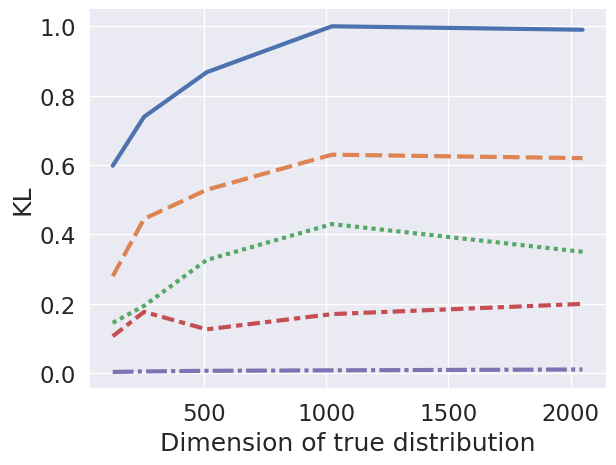
\includegraphics[height=4.5cm]{imgs/hmm/cat-kl.png}
\caption{}
\end{subfigure}
\begin{subfigure}[t]{0.43\textwidth}
\centering
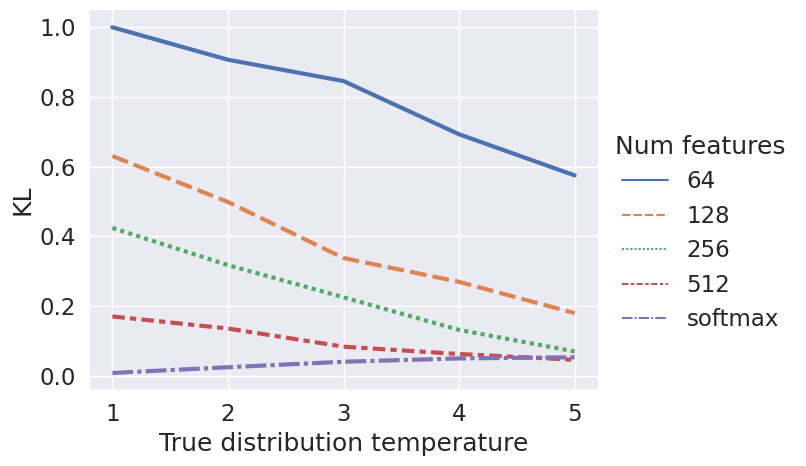
\includegraphics[height=4.5cm]{imgs/hmm/cat-temp-kl.png}
\caption{}
\end{subfigure}
\caption{\label{fig:cat-kl}The KL between the true synthetic categorical distribution and learned linearized model, measuring the effect of: (a) The dimension of the true distribution $|\mcL|$. The number of queries is held constant at 128 and temperature at $\tau=1$, while the dimension of the true distribution 
and the number of features in the linearized model is varied. (b) The temperature of the true distribution $\tau$. The number of queries is held constant at 128 and keys at 1024, while the temperature of the true distribution 
and the number of features is varied.}
\end{figure*}

\section{Results}
% Categorical
\paragraph{Preliminary: Categoricals}
We first consider how well the kernel softmax approximation 
fits synthetically generated categorical data.
Figure~\ref{fig:cat-kl} (a) illustrates the relationship between the number of features $N$ and the state space size of the discrete softmax distribution. In all cases, a randomly initialized softmax model $K_\SM$ was able to achieve $< 0.05$ KL, whereas the approximate models $K_{\textrm{pos}}$ performed worse. The KL between the true and learned distributions at convergence decreases with more features, which lends the model more expressivity but increases the computational cost.
In Figure~\ref{fig:cat-kl} (b), we compare approximate softmax models at varying temperatures. We see that $K_{\textrm{pos}}$ is able to achieve lower KL as the temperature of the true distribution increases, resulting in a higher entropy true distribution.

These experiments show that the ratio between the size of the distribution and the number of features balances accuracy and efficiency.
There is a consistent gain in modeling flexibility with more features, but they all lag 
behind softmax in this setting.

% PTB LM HMM
\begin{table}[!t]
\centering
\begin{tabular}{lrr}
\toprule
Model & Val & Test\\
\midrule
%GPT-3 & - & 20.5 \\
BERT-Large-CAS & 36.1 & 31.3\\
%AWD-LSTM-DOC & 54.1 & 52.4\\
AWD-LSTM & 60.0 & 57.3\\
VL-HMM $|\mcL|=2^{15}$ & 125.0 & 116.0\\
HMM $|\mcL|=1024$ & 182.5 & 170.1\\
LHMM $|\mcL|=1024$ & 179.7 & 165.9\\
LHMM $|\mcL|=2048$ & 172.3 & 160.2\\
LHMM $|\mcL|=4096$ & 173.7 & 159.8\\
\bottomrule
\end{tabular}
\caption{\label{tbl:hmm-ppl}
Validation and test perplexities on \textsc{Ptb}.
All LHMMs all use a fixed number of features, $N = 512$.
}
\end{table}
\paragraph{Hidden Markov Model}

\begin{comment}
Table~\ref{tbl:hmm-ppl} shows the results for language modeling with HMMs on \textsc{Ptb}.
The Low-rank HMMs (LHMM) achieve equal performance with their softmax counterparts at a
fraction of the computational cost, as the LHMM takes time $O(T|\mcL|N)$
while the softmax HMM takes time $O(T|\mcL|^2)$, with $|\mcL|=1024$ and $N=512$.
However, while we are able to train larger models efficiently, as expected,
these models are significantly outperformed by neural autoregressive approaches.
A more fair comparison is with the VL-HMM \citep{chiu2020scaling},
a large HMM model that exploits fixed sparsity patterns in the model and scales to 64K states.
We believe with some of these same approaches the LHMM could scale to larger sizes as well.

Table~\ref{tbl:hmm-ppl-states} compares LHMMs to standard softmax HMMs.
We find that for a fixed number of features $n=512$,
LHMMs are able to match the performance of softmax HMMs with the same state size,
up to $|\mcL|=1024$ states.
As we increase the number of states further,
while still keeping the number of features fixed at $N=512$,
the perplexity continues to improve up until $|\mcL|=4096$,
where performance is the same as the LHMM with $|\mcL|=2048$.
Further examining the relationship between the number of labels $|\mcL|$ and features $N$,
Figure~\ref{fig:hmm-ppl-features} shows that for a fixed number of states,
$|\mcL|=512$, performance remains the same after halving the number of features to 256,
but degrades as we decrease the number of features, once $N < 256$.

Table~\ref{tbl:hmm-ablation} shows the results of ablations for the LHMM.
Ablations are conducted by independently on a base LHMM with 256 states and features.
Constraining embeddings to $l_2$ norm 1 leads to very similar performance.
We find that fixing the feature map and not learning through it results in a loss in performance.
Additionally, we find that the form of the feature map impacts performance as well,
with $\phi_{\textrm{pos}}$ outperforming both $\phi_\ReLU$ and $\phi_{\exp}$.
\end{comment}

% Scaling results: No dropout, dropout, band
Figure~TBD shows the results for language modeling with HMMs on \textsc{PTB}.
Low-rank HMMs (LHMM) are able to match the performance of unconstrained softmax HMMs
at a fraction of the computational cost.
% move this to methods?
As the low-rank transition structure replaces the $O(\mcL^2)$ computation
in inference with 2 $O(\mcL N)$ operations, 

Table~TBD shows that HMMs do not out-perform LSTM-based models,
as seen in previous work \citep{chiu2020scaling}.
% Comparison to LSTM and VL-HMM
Additionally, for language modeling on \textsc{PTB},
LHMMs are outperformed by VL-HMMs \citep{chiu2020scaling} in both accuracy and speed.
This is expected, as the specific block-sparse emission constraint applied in VL-HMMs
requires very strong assumptions, and therefore gives very strong speedups as well
as regularization.
% Timing

\begin{table}[!t]
\centering
\begin{tabular}{lrrcrr}
\toprule
& \multicolumn{2}{c}{LHMM} && \multicolumn{2}{c}{Softmax HMM}\\
\cmidrule{2-3} \cmidrule{5-6}
$|\mcL|$ & Train & Val && Train & Val\\
\midrule
256  & 167 & 205 && 179 & 215\\
512  & 146 & 192 && 156 & 197\\
1024 & 136 & 180 && 137 & 183 \\
2048 & 120 & 172 && -   & -\\
4096 & 126 & 174 && -   & - \\
\bottomrule
\end{tabular}
\caption{\label{tbl:hmm-ppl-states}
Perplexities on \textsc{Ptb} for the Softmax HMM and LHMM with a fixed number of features, $N = 512$.
Softmax HMMs with state sizes $|\mcL|$ greater than 1024 are not run due to computational constraints.
}
\end{table}

\begin{figure}[t]
\centering
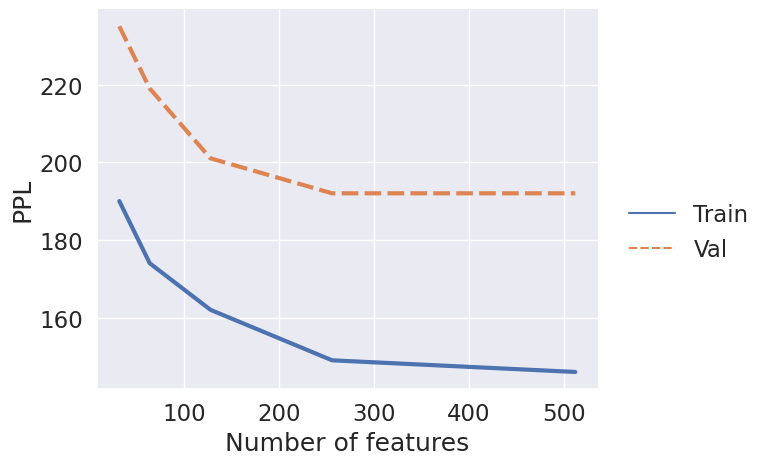
\includegraphics[height=4.5cm]{imgs/hmm/hmm-ppl-features.png}
\caption{
\label{fig:hmm-ppl-features}
Perplexities on \textsc{Ptb} for an LHMM with a varying number of features $N$ and fixed number of states $|\mcL|=512$.
}
\end{figure}

\begin{figure}[t]
\centering
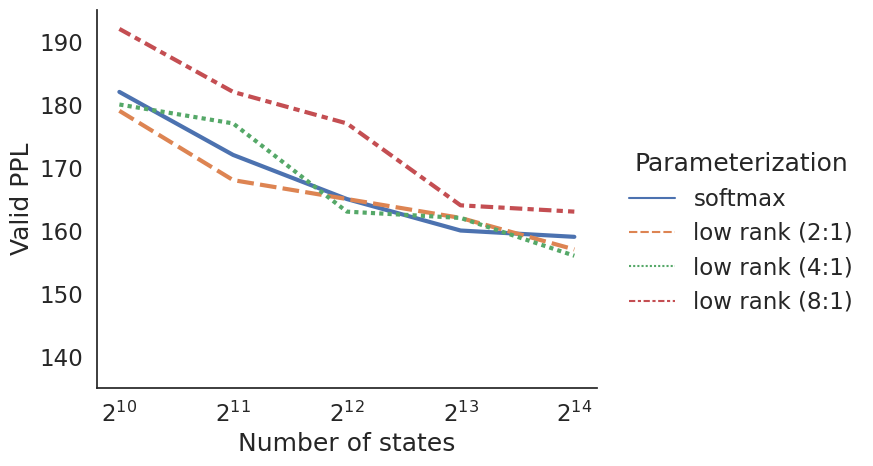
\includegraphics[height=4.5cm]{imgs/hmm/lhmm-states-features.png}
\caption{
\label{fig:hmm-ppl-features}
Perplexities on \textsc{Ptb} for an LHMM with a varying number of features $N$ and fixed number of states $|\mcL|=512$.
}
\end{figure}

\begin{figure}[t]
\centering
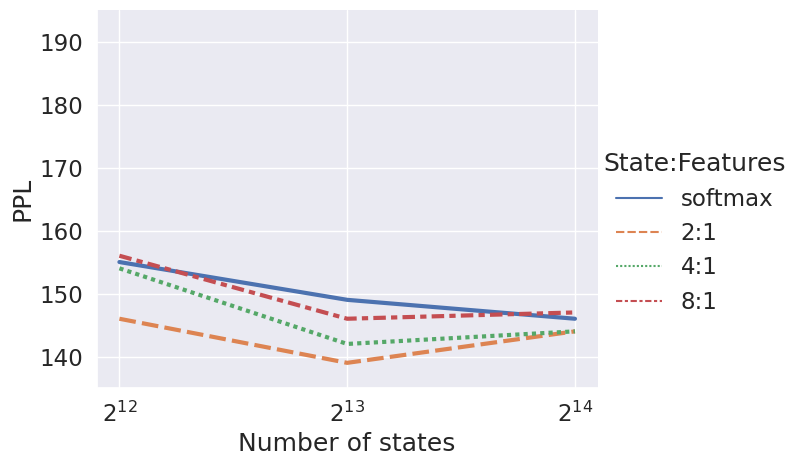
\includegraphics[height=4.5cm]{imgs/hmm/lhmm-states-features-dropout.png}
\caption{
\label{fig:hmm-ppl-features}
Perplexities on \textsc{Ptb} for an LHMM with a varying number of features $N$ and fixed number of states $|\mcL|=512$.
}
\end{figure}

\begin{figure}[t]
\centering
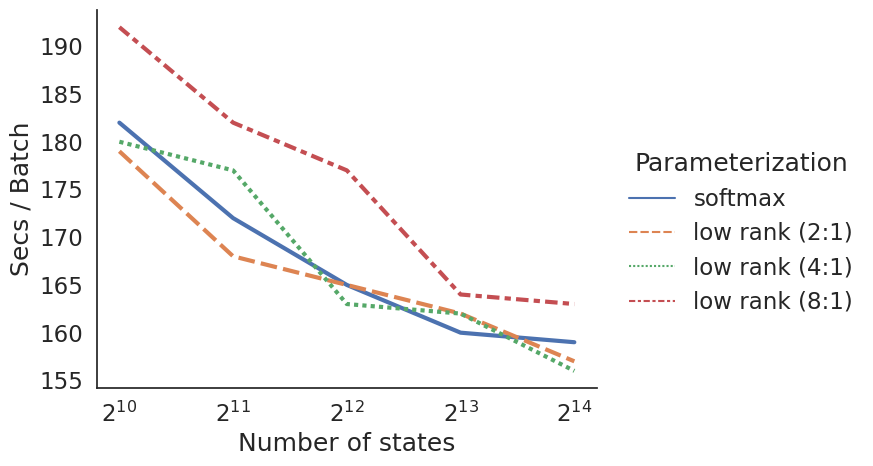
\includegraphics[height=4.5cm]{imgs/hmm/lhmm-states-features-speed.png}
\caption{
\label{fig:hmm-ppl-features}
Perplexities on \textsc{Ptb} for an LHMM with a varying number of features $N$ and fixed number of states $|\mcL|=512$.
}
\end{figure}

\begin{table}[!t]
\centering
\begin{tabular}{lrr}
\toprule
Model & Train & Val \\
\midrule
LHMM                         & 173 & 213\\
\quad + embedding normalization      & 174 & 215 \\
\quad + random $\phi_\textrm{pos}$ & 182 & 222\\
\quad + $\phi_{\exp}$              & 338 & 349\\
\quad + $\phi_\ReLU$               & 185 & 223\\
\bottomrule
\end{tabular}
\caption{\label{tbl:hmm-ablation}
Ablations for the embedding normalization and feature map on \textsc{Ptb} in a LHMM with a fixed number of states $|\mcL| = 256$ and features $n=256$.
We perform each ablation independently.
}
\end{table}

% PTB PARSING PCFG
\paragraph{Context-Free Grammars}

For syntactic language modeling on \textsc{Ptb}, we found that our kernel methods achieve similar performance to softmax PCFGs, as shown in Table~\ref{tbl:cky}, with an improvement in complexity. For example, when $|\mcN|=30$ and $|\mcP|=60$, we can achieve within 5 PPL points using only 4 features, and comparable results using 8 features. As we scale up the number of nonterminals and preterminals to 100 and 200, kernel PCFG stays competitive with a lower computational complexity (since $N < |\mcN|$). These experiments demonstrate the importance of scale with a nearly more than 50 point gain in perplexity over a strong starting model. 

% PCFG ablation studies
In Table~\ref{tbl:cky-ablation}, we consider the effects the mixed kernel parameterization, i.e. of replacing the softmax kernel with the approximate kernel. In particular we consider different combinations of preterminal / nonterminal tails $B\ C\in \mcN\times\mcN$, $B\ C\in \mcN\times\mcP$, $B\ C\in \mcP\times\mcN$, and $B\ C\in \mcP\times\mcP$ (our main model only factorizes nonterminal / nonterminal tails). Table~\ref{tbl:cky-ablation} shows that we get the best perplexity when we only use $K$ on $B\ C\in \mcN\times\mcN$, and use softmax kernel $K_\SM$ for the rest of the space. This fits with previous observations that when the label space $|\mcL|$ is large, the kernel approximation hurts performance. \footnote{In this particular ablation study, the size of $\mcN\times\mcN$ is only one-ninth of the total state space size $\{\mcN \cup \mcP\}\times \{\mcN \cup \mcP\}$.}


Figure~\ref{fig:example_production} shows the entropy distribution of the production rules $H(P(B\ C | A))$ for both using softmax kernel and the approximation. We also visualized the distributions for a subset of $A$'s in Appendix~\ref{sec:pcfgvismore}. The average entropies of the two distributions are close . Besides, under this setting, $P(B\ C \in \mcN \times \mcN| A)$ are close for both kernels as well (softmax 0.20, linear 0.21), eliminating the possibility that the kernel model simply learns to avoid using $B\ C \in \mcN \times \mcN$ (such as by using a right-branching tree). 






\begin{table}[!t]
\centering
\begin{tabular}{@{}lllrr@{}}
\toprule
$|\mcN|$ & $|\mcP|$ & Model & $N$ &  PPL \\
\midrule
30  & 60    & Neural PCFG &\hspace{-1.7cm}\citep{kim2019cpcfg}  & 252.6\\
    &       & Neural PCFG (reimpl.) & - & 249.62    \\
    &       & Kernel PCFG       & 4 & 255.42          \\
    &       & Kernel PCFG       & 8 &  247.02         \\
    &       & Kernel PCFG       & 16 & 250.59        \\
% 32>30, so maybe we shouldn't use this at all    &       & Kernel PCFG       & 32 &           \\
\midrule
60  & 120   & Neural PCFG (reimpl.) & - & 234.01\\ % this number is much higher than val, not sure why
    &       & Kernel PCFG       & 16& 217.24 \\
    &       & Kernel PCFG       & 32& 213.81 \\
\midrule
100 & 200   & Neural PCFG (reimpl.) & - &  191.08    \\
    &       & Kernel PCFG       & 32& 203.47 \\
    &       & Kernel PCFG       & 64& 194.25 \\
%    &       & Kernel PCFG       & 90& \\
\bottomrule
\end{tabular}
\caption{\label{tbl:cky}
Test perplexities of PCFG models on \textsc{Ptb}. All models presented here do not use continuous latent variables.
}
\end{table}

\begin{table}[!htp]
\centering
\begin{tabular}{lllrr}
\toprule
\multicolumn{4}{c}{Kernel for $B\ C $} & \multirow{2}{*}{PPL}\\
\cmidrule{1-4}
$\mcN\times \mcN$ & $\mcN\times\mcP$  & $\mcP\times\mcN$ & $\mcP\times\mcP$ \\
\midrule
  Softmax & Softmax & Softmax & Softmax & 243.19\\
  Linear & Softmax & Softmax & Softmax & 242.72\\
  Linear & Linear & Linear & Softmax &  259.05 \\
  Linear & Linear & Linear & Linear & 278.60 \\
\bottomrule
\end{tabular}
\caption{\label{tbl:cky-ablation}
Ablation studies of PCFG. The perplexities are evaluated on the validation set of \textsc{Ptb}. Here we use $|\mcN|=30$, $|\mcP|=60$, and 16 features for linearlized kernel.
}
\end{table}


\begin{figure*}[!htp]
  \centering
  \begin{subfigure}[t]{0.45\textwidth}
  \centering
  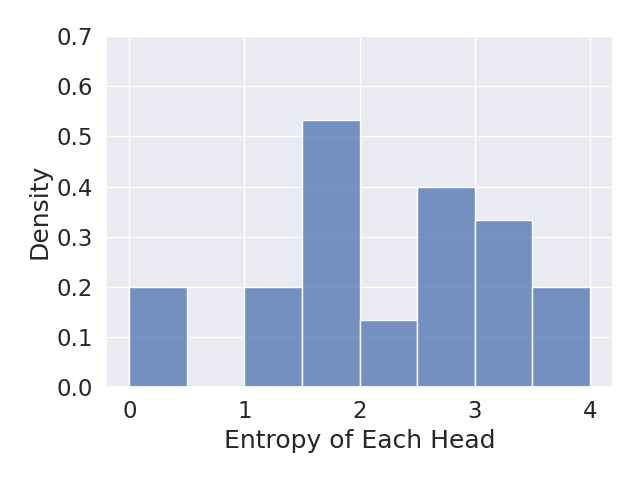
\includegraphics[width=0.9\textwidth]{imgs/softmax/entropy.png}
  \caption{Softmax Kernel $K_\SM$}
  \end{subfigure}
  \begin{subfigure}[t]{0.45\textwidth}
  \centering
  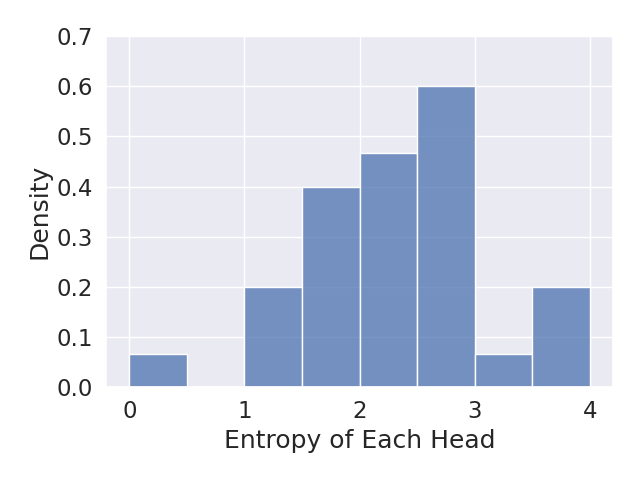
\includegraphics[width=0.9\textwidth]{imgs/rff/entropy.png}
  \caption{Linearized Kernel $K_{\textrm{pos}}$}
  \end{subfigure}
  \caption{\label{fig:example_production}Histogram of entropies of $P(B\ C\mid A)$. The average entropy is 2.26 for softmax kernel and 2.34 for linearized kernel. We use $|\mcN|=30$, $|\mcP|=60$, and $N=16$ for linearized kernel. Example visualizations of probabilities $P(B\ C|A)$ for particular $A$'s can be found in Appendix~\ref{sec:pcfgvismore}.}
\end{figure*}

\section{Related Work}

Work on linear time and space attention has made tremendous progress, coming close to \citep{shen2018linearattn,katharopoulos2020lineartransformer,wang2020linformer} or matching \citep{choromanski2020performer,peng2021rfa} the performance of regular softmax attention, which takes time quadratic in the length of a sequence.
This work builds upon prior work in viewing attention through the lens of a kernel \citep{tsai2019kernelattn}, as well as kernel-based approximations for sampled softmax \citep{blanc2018sampledsoftmax,rawat2019sampledsoftmax}.
We draw our kernel parameterizations from \citet{choromanski2020performer}, and extend their application to the structured prediction setting.

Kernel embeddings of graphical models \citep{song2011kernelbp}
have been applied to a variety of settings:
HMMs \citep{song2010kernelhmm}
and latent trees \citep{song2011kerneltree},
where in both cases a spectral algorithm was used for learning. There is also a large family of work on spectral methods for structured prediction, on HMMs \citep{hsu2012spectral} as well as PCFGs \citep{cohen2012lpcfg,clark-fijalkow-2020-consistent}. As a member of the family of method of moments estimators, spectral methods are typically not robust to model misspecification \citep{ruffini2017mom}. Our approach relies on maximum likelihood estimation, which finds the KL-projection of the true distribution onto our hypothesis class and is therefore more robust to misspecification.
Additionally, we capitalize on modern parallel hardware in order to scale to much larger models than previously considered.

\section{Conclusion}

This work improves the scaling of structured models by  establishing the effectiveness of kernel decomposition for inference. We show that recent work in efficient attention with kernel methods \citep{choromanski2020performer,peng2021rfa} allows us to embed inference in structured models through a kernel approximation of softmax. Embedded inference allows us to obtain a reduction of a factor of the number of labels in the asymptotic complexity of marginalization. Our approach applies to a wide class of models, including HMMs and PCFGs. Through our experiments on synthetic data and language modeling, we demonstrate an effective approach for overcoming the practical difficulty of applying kernels in high dimensional, structured spaces by targeting and kernelizing model components that bottleneck computation. Future work includes the extension of embedded inference to models where exact inference is intractable, and a theoretical characterization of the limitations of the method.


\section*{References}
\citep{choromanski2020performer}
References follow the acknowledgments. Use unnumbered first-level heading for
the references. Any choice of citation style is acceptable as long as you are
consistent. It is permissible to reduce the font size to \verb+small+ (9 point)
when listing the references.
Note that the Reference section does not count towards the page limit.
\medskip

\bibliography{bib}
\bibliographystyle{plainnat}

{
\small

[1] Alexander, J.A.\ \& Mozer, M.C.\ (1995) Template-based algorithms for
connectionist rule extraction. In G.\ Tesauro, D.S.\ Touretzky and T.K.\ Leen
(eds.), {\it Advances in Neural Information Processing Systems 7},
pp.\ 609--616. Cambridge, MA: MIT Press.

[2] Bower, J.M.\ \& Beeman, D.\ (1995) {\it The Book of GENESIS: Exploring
  Realistic Neural Models with the GEneral NEural SImulation System.}  New York:
TELOS/Springer--Verlag.

[3] Hasselmo, M.E., Schnell, E.\ \& Barkai, E.\ (1995) Dynamics of learning and
recall at excitatory recurrent synapses and cholinergic modulation in rat
hippocampal region CA3. {\it Journal of Neuroscience} {\bf 15}(7):5249-5262.
}

%%%%%%%%%%%%%%%%%%%%%%%%%%%%%%%%%%%%%%%%%%%%%%%%%%%%%%%%%%%%
\section*{Checklist}

%%% BEGIN INSTRUCTIONS %%%
The checklist follows the references.  Please
read the checklist guidelines carefully for information on how to answer these
questions.  For each question, change the default \answerTODO{} to \answerYes{},
\answerNo{}, or \answerNA{}.  You are strongly encouraged to include a {\bf
justification to your answer}, either by referencing the appropriate section of
your paper or providing a brief inline description.  For example:
\begin{itemize}
  \item Did you include the license to the code and datasets? \answerYes{See Section~\ref{gen_inst}.}
  \item Did you include the license to the code and datasets? \answerNo{The code and the data are proprietary.}
  \item Did you include the license to the code and datasets? \answerNA{}
\end{itemize}
Please do not modify the questions and only use the provided macros for your
answers.  Note that the Checklist section does not count towards the page
limit.  In your paper, please delete this instructions block and only keep the
Checklist section heading above along with the questions/answers below.
%%% END INSTRUCTIONS %%%

\begin{enumerate}

\item For all authors...
\begin{enumerate}
  \item Do the main claims made in the abstract and introduction accurately reflect the paper's contributions and scope?
    \answerTODO{}
  \item Did you describe the limitations of your work?
    \answerTODO{}
  \item Did you discuss any potential negative societal impacts of your work?
    \answerTODO{}
  \item Have you read the ethics review guidelines and ensured that your paper conforms to them?
    \answerTODO{}
\end{enumerate}

\item If you are including theoretical results...
\begin{enumerate}
  \item Did you state the full set of assumptions of all theoretical results?
    \answerTODO{}
	\item Did you include complete proofs of all theoretical results?
    \answerTODO{}
\end{enumerate}

\item If you ran experiments...
\begin{enumerate}
  \item Did you include the code, data, and instructions needed to reproduce the main experimental results (either in the supplemental material or as a URL)?
    \answerTODO{}
  \item Did you specify all the training details (e.g., data splits, hyperparameters, how they were chosen)?
    \answerTODO{}
	\item Did you report error bars (e.g., with respect to the random seed after running experiments multiple times)?
    \answerTODO{}
	\item Did you include the total amount of compute and the type of resources used (e.g., type of GPUs, internal cluster, or cloud provider)?
    \answerTODO{}
\end{enumerate}

\item If you are using existing assets (e.g., code, data, models) or curating/releasing new assets...
\begin{enumerate}
  \item If your work uses existing assets, did you cite the creators?
    \answerTODO{}
  \item Did you mention the license of the assets?
    \answerTODO{}
  \item Did you include any new assets either in the supplemental material or as a URL?
    \answerTODO{}
  \item Did you discuss whether and how consent was obtained from people whose data you're using/curating?
    \answerTODO{}
  \item Did you discuss whether the data you are using/curating contains personally identifiable information or offensive content?
    \answerTODO{}
\end{enumerate}

\item If you used crowdsourcing or conducted research with human subjects...
\begin{enumerate}
  \item Did you include the full text of instructions given to participants and screenshots, if applicable?
    \answerTODO{}
  \item Did you describe any potential participant risks, with links to Institutional Review Board (IRB) approvals, if applicable?
    \answerTODO{}
  \item Did you include the estimated hourly wage paid to participants and the total amount spent on participant compensation?
    \answerTODO{}
\end{enumerate}

\end{enumerate}

%%%%%%%%%%%%%%%%%%%%%%%%%%%%%%%%%%%%%%%%%%%%%%%%%%%%%%%%%%%%

\appendix

\section{Appendix}

Optionally include extra information (complete proofs, additional experiments and plots) in the appendix.
This section will often be part of the supplemental material.

\end{document}
